\section{Metodi: mappare gli elementi legnosi in alveo}
Le piante che caratterizzano l'ambiente ripario nell'area di studio, \emph{Salix spp.} e \emph{Populus nigra}, sono in grado di riprodursi tramite la dispersione di semi;
tuttavia, la riproduzione vegetativa a partire da elementi legnosi, quali pezzi di tronchi, piante e arbusti e accumuli di legname, ottiene un successo maggiore e costituisce il fondamentale meccanismo di propagazione, formazione ed espansione delle isole \squarecite{Gurnell:2001-island-formation}.
\\
La dimensione degli elementi legnosi è molto variabile: da frammenti vegetativi a piccole piante deposte sulle barre, da alberi alti diversi metri a consistenti accumuli di legname.
Tra le immagini a disposizione, solo le ortofoto, le immagini \Pl{} e le immagini \WV{} hanno una risoluzione sufficientemente elevata da permettere il riconoscimento del legno.
\\
Si è proceduto quindi digitalizzando manualmente le posizioni di tutti gli elementi legnosi in una porzione di alveo compresa tra il tratto~7 e l'8 per le immagini ad alta risoluzione del~2010-08, 2013-10-22, 2014-10-31, 2015-08-13 e~2017-06-26/08-02; queste hanno un errore di georeferenziazione nell'ordine di una decina di centimetri.
\\
Non si sono digitalizzate altre aree oltre a quella scelta poiché sembrano essere meno ricche di legno; non è stato possibile implementare un sistema di riconoscimento automatico o semi-automatico neanche per le immagini satellitari multibande poiché il colore degli elementi legnosi è molto variabile e non è stato possibile legarlo con una combinazione di diverse bande come nel caso delle isole con l'NDVI.
Non sono state considerate le ortofoto del~2005-05 e~2011-06-26/07-02 poiché la prima non ha una qualità tale da poter distinguere bene gli elementi più piccoli e la seconda non è perfettamente georeferenziata (tentativi di rigeoreferenziazione come quelli eseguiti precedentemente sulle immagini \AST{} hanno dato risultati poco soddisfacenti).
\\
Sono stati digitalizzati più di un migliaio di elementi legnosi per ogni immagine considerata.
La \cref{fig:digitalizzazione-legno} mostra l'area dove si è effettuata la digitalizzazione e un esempio di individuazione degli elementi legnosi.
%
\begin{figure}
	\centering
	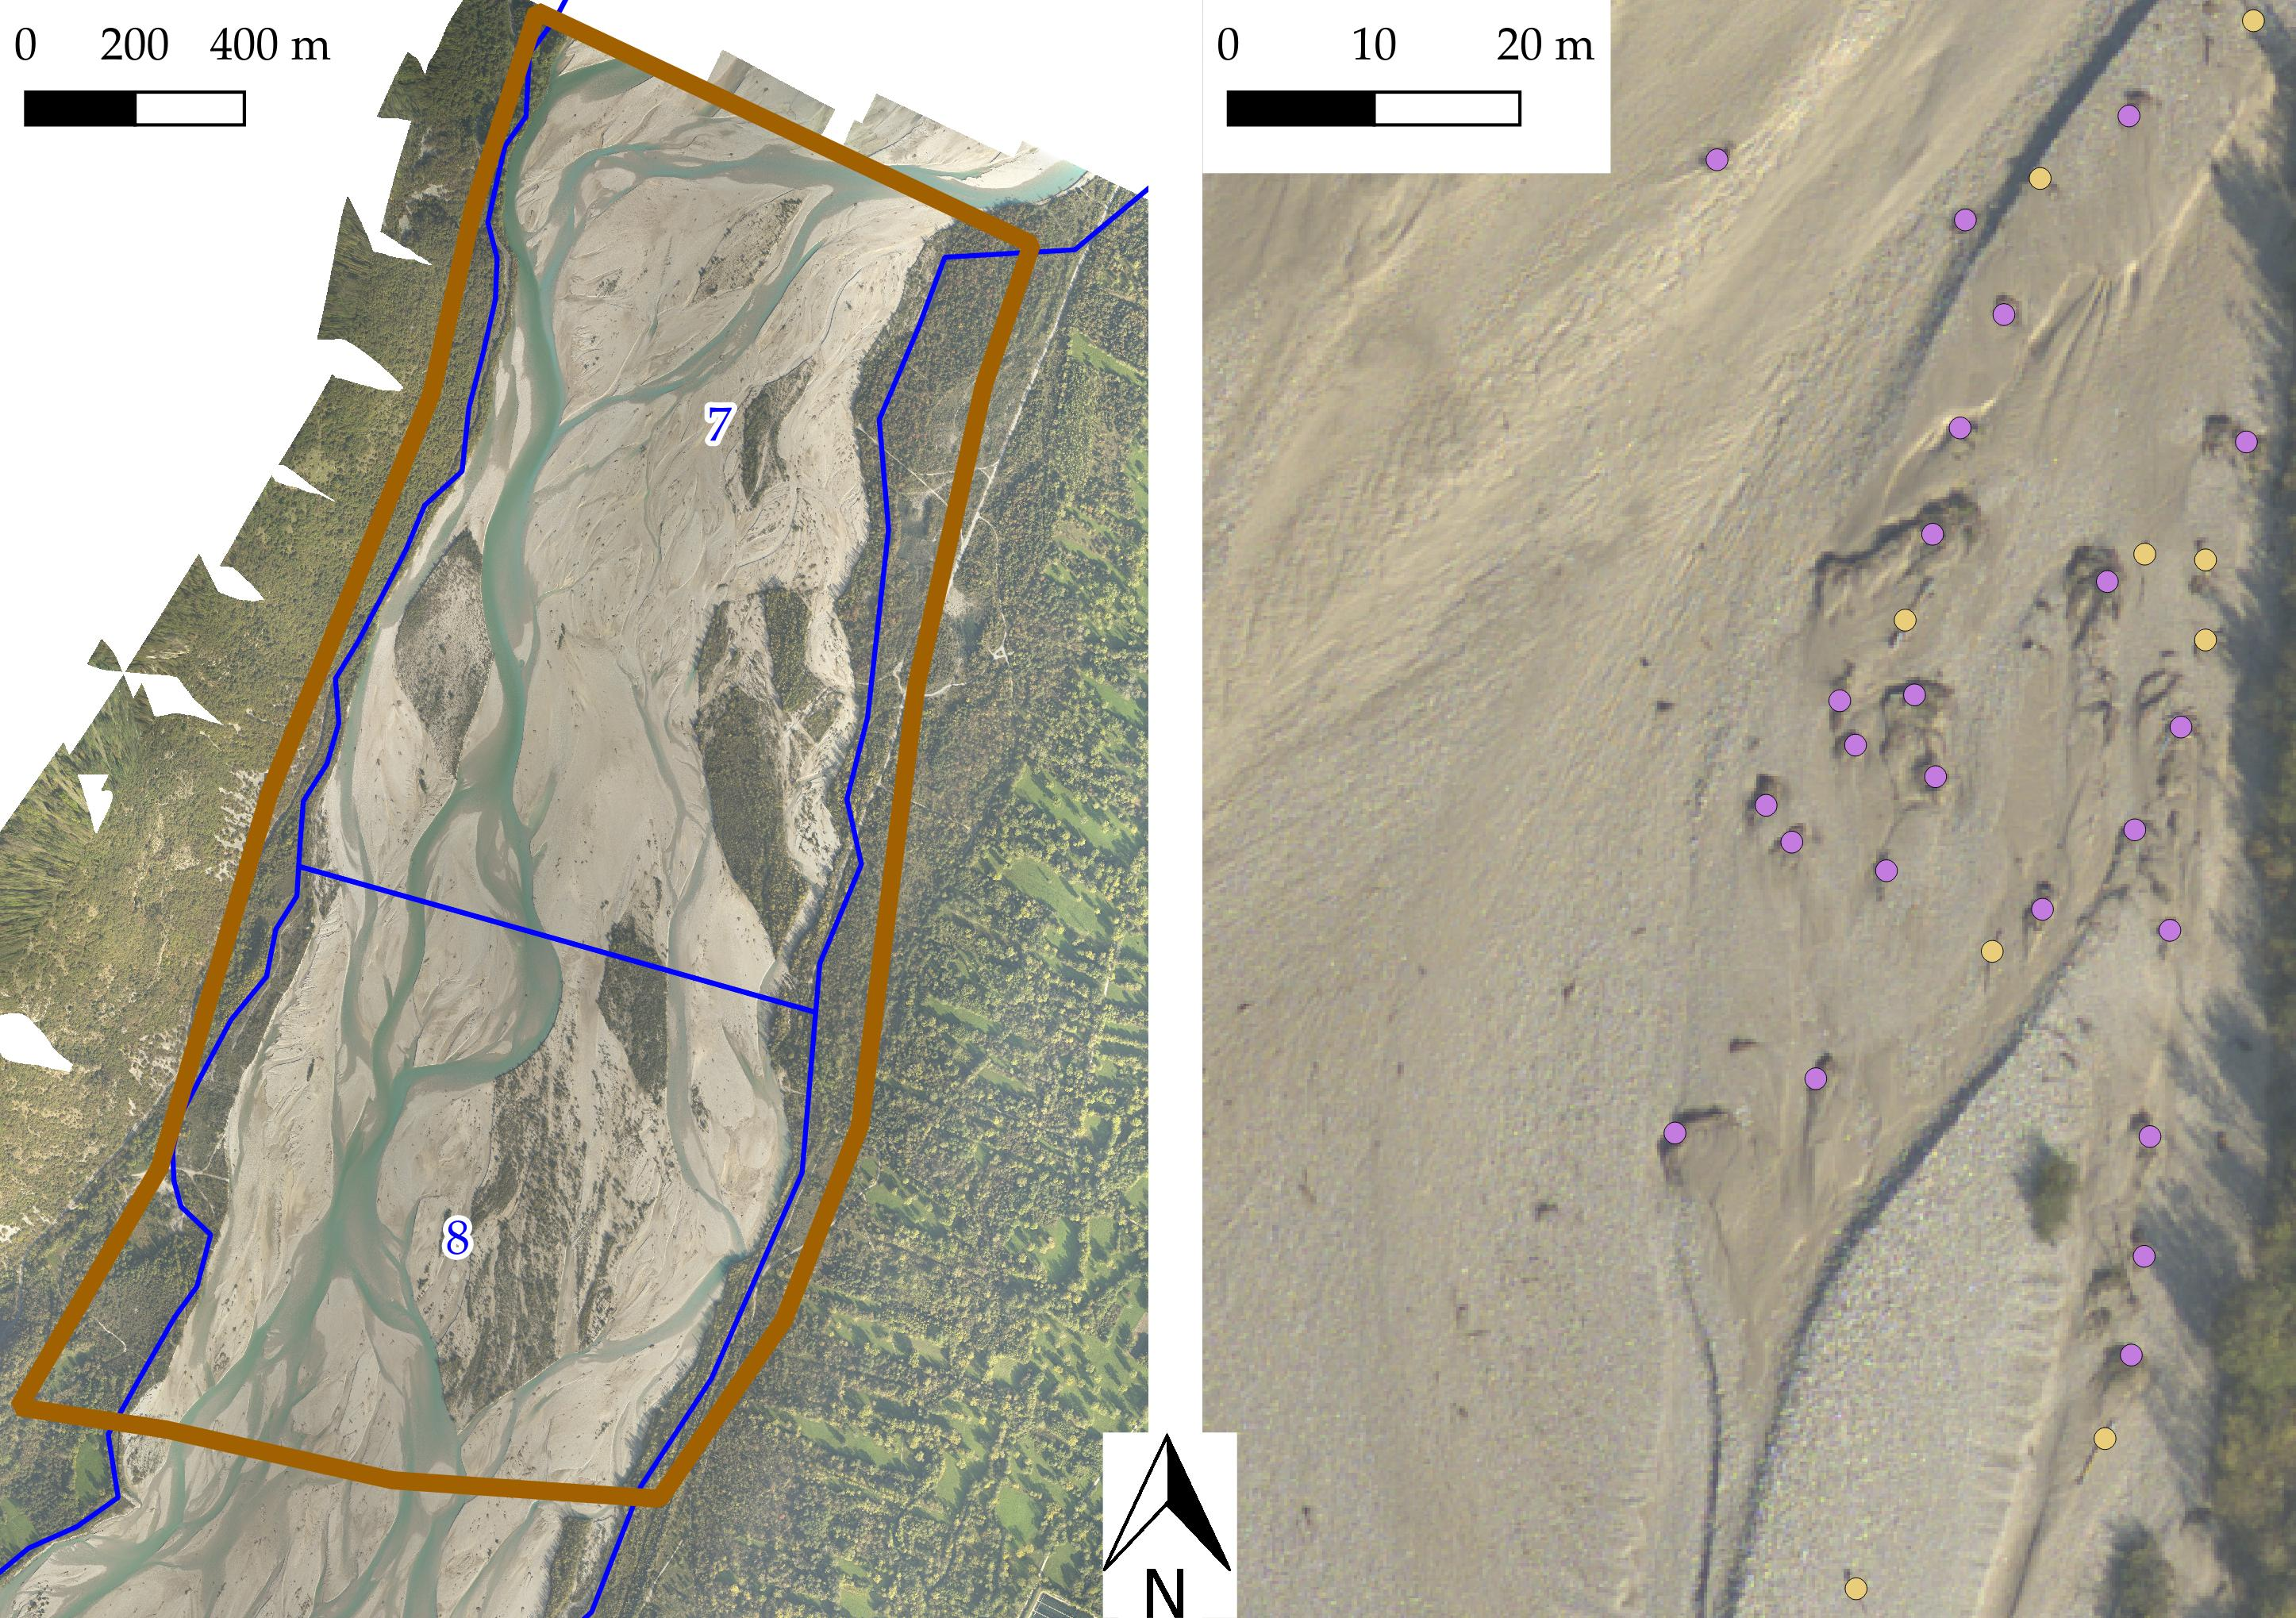
\includegraphics[width = \textwidth]{files/digitalizzazione_legno.jpeg}
	\caption[area dove sono stati digitalizzati gli elementi legnosi]{a sinistra l'area di digitalizzazione degli elementi legnosi (in marrone) e la maschera computazionale divisa in tratti (in blu); a destra un esempio di digitalizzazione in cui sono stati distinti i tronchi (in arancione) dagli accumuli (in viola); sullo sfondo è presente l'ortofoto del~2013-10-22.}
	\label{fig:digitalizzazione-legno}
\end{figure}
%

In seguito per ogni digitalizzazione si è calcolata la distanza tra ogni punto e quello più vicino nella digitalizzazione successiva. Ad esempio, per ogni elemento legnoso nella mappa del~2014-10-31 è stato ottenuta la distanza dall'elemento legnoso più prossimo nella mappa del~2015-08-13.
Se la distanza è sufficientemente bassa, si considera l'elemento legnoso nella prima digitalizzazione come non mobilitato; se la distanza è elevata, il legno mappato nelle due digitalizzazioni o non è il medesimo o è stato spostato dalle piene.
Gli elementi che non sono mobilitati hanno, negli anni seguenti, la possibilità di diventare prima arbusti, poi alberi ed infine isole.
\\
Infine per le ortofoto associate ad un rilievo LiDAR (il~2010-08 e il~2013-10-22) si è ottenuta la quota di ogni punto rispetto al DEM privo dell'effetto della pendenza (questo viene calcolato sottraendo al DEM la quota media in quella zona, cioè eliminando l'effetto della pendenza; in questo modo le quote sono riferite ad uno zero locale e mostrano chiaramente zone incise, come i canali, e zone elevate, come le barre).
